\documentclass[conference]{IEEEtran}

%% CITATIONS, REFERENCES ETC. %%
\usepackage[draft]{fixme}
\fxsetup{footnote, margin=false}

\usepackage{cite}

\usepackage[nolist,nohyperlinks]{acronym}
\begin{acronym}
  \acro{ip}[IP]{Internet Protocol}
\end{acronym}

%%% Local Variables:
%%% mode: latex
%%% TeX-master: "../paper"
%%% End:


\hyphenation{op-tical net-works semi-conduc-tor}

\usepackage{url}

%% GRAPHICS, TABLES ETC. %%
\usepackage[pdftex, final]{graphicx}
\graphicspath{{./figures/}}
\DeclareGraphicsExtensions{.pdf,.jpeg,.png}

\usepackage{tikz}

\usepackage{diagbox}

%% MATH, CODE ETC. %%
\usepackage{amsmath}
\interdisplaylinepenalty=2500

\usepackage{amssymb}

%\usepackage{listings}

\begin{document}

\title{Paper title goes here}

\author{
  \IEEEauthorblockN{First~Author, Second~Author, Third~Author}
  \IEEEauthorblockA{Department\\
    University, Country\\
    Email: \{one, two, three\}@example.com
  }
}
\maketitle


\begin{abstract}
Abstract goes here.
\end{abstract}

\section{First section}
\label{sec:first_section}

This is the first paragraph, with an acronym: \ac{ip}.

This is the second paragraph, with a reference to \cite{ref}.
\begin{figure}[htb]
  \centering
  \resizebox{2,5in}{!}{%
    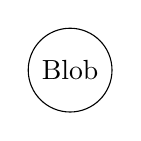
\begin{tikzpicture}
      \node[draw, circle] (blob) {Blob};
    \end{tikzpicture}
  }
  \caption{
    This is a blob
  }
  \label{fig:blob}
\end{figure}

\subsection{First subsection}
\label{sec:first_subsection}

\begin{align}
  \label{eq:1}
  A & = B \\
  \label{eq:2}
  1 + 1 & = 2
\end{align}

\section{Second section}
\label{sec:second_section}

\begin{figure}[htb]
  \centering
  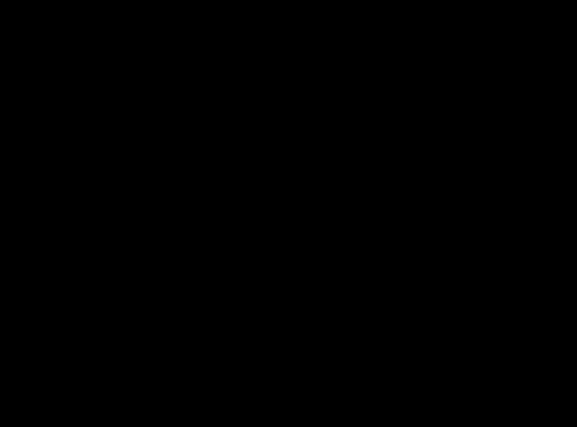
\includegraphics[width=2.5in]{figures/blob}
  \caption{
    This is a black blob
  }
  \label{fig:picture}
\end{figure}

%% BIBLIOGRAPHY %% 
\bibliographystyle{IEEEtran}
\bibliography{IEEEabrv,bib/paper}

\end{document}

%%% Local Variables:
%%% mode: latex
%%% TeX-master: t
%%% End: